%!TEX root = ../../Main.tex
\graphicspath{{Chapters/Indledning/}}
%-------------------------------------------------------------------------------

\chapter{Subset selection}

This chapter will address the subject Subset selection. Subset selection concerns with selecting or shrinking the coefficients of features to make the model more interpretable and in some cases to predict better.

Linear models are simple and can be interpreted because it usually has a small number of coefficients.
In cases where the number of predictors is bigger than the number of samples, we can’t use the full least squares, because the solutions is not even defined. In such cases we must reduce the number of features to be able to obtain a solution. It is also very important to not fit your data too hard which regularize, or selection of features also helps with. Along the same lines, when we have a small number of features the model becomes more interpretable.  

There exist many different methods to perform subset selection. One of the methods to select the most important features regarding a specific response is called best subset selection. This is where we identify a subset of the predictors that is most related to the response. 

\section{Best subset selection}

Best subset selection algorithm is a simple algorithm used to understand which predictors are mostly linked to the responds. To perform best subset selection, we fit a separate least squares regression for each possible combination. It starts out by fitting all p models that contain exactly one predictor, then fitting all p models that contain exactly two predictors and so forth. The number of models to fit can be calculated like this: 
\begin{equation}
(\frac{p}{k})=\frac{p!}{k!(p-k)!}\label{Best_subset_models_eq}
\end{equation}
Where p is the number of all predictors, and k is the number of predictors in the subset. After all possible combinations of p models has been fitted, we then look at the resulting model, with the goal of identifying the best one. \\
Best subset selection algorithm can be divided into three steps:

\begin{enumerate}
	\item Let $M_0$ denote the \textit{null model}, which contain no predictors. This model simply predicts the sample mean for each observation.
	
	\item For k=1,2,...p:
	\begin{enumerate}
		\item Fit all $\binom{p}{k}$ models that contain exactly \textit{k} predictors.
		
		\item Pick the best among these $\binom{p}{k}$ models, and call it $M_k$. Here \textit{best} is defined as having the smallest RSS, or equivalently largest $R^2$
	\end{enumerate}
	\item Select a single best model from among $M_0$,...,$M_p$ using crass-validated prediction error, AIC, BIC or adjusted $R^2$
\end{enumerate}


The task of to selecting the best subset model, must be performed with care, because RSS decreases monotonically and the $R^2$ increases monotonically, as the number of features included in the models increases. So, if we use these statistics, we will always end up med the model involving all the variables. 
Another problem with a low RSS or a high $R^2$ is that it only indicates a model with a low training error. And a low training error does not equal a low test error. So, for those reasons we need to use cross-validation, AIC, BIC or adjusted $R^2$. 

\section{Stepwise Selection}
If the number of predictors p gets too large, best subset selection algorithm cannot be applied for computational reasons. Another reason why best subset selection is not always the best algorithm to select at subset, is for statistical reasons if the p is too large. Then there is a higher chance of finding models that look good on the training data, even though they might not have any predictive power on future data. 
For these reasons, stepwise methods, which explore a far more restricted set of models, are attractive alternatives to best subset selection. 

In this section we'll touch upon two different stepwise selection methods; the forward stepwise selection method and the backwards stepwise selection method.

\subsection{Forward stepwise selection}
Forward stepwise selection method is very similar to the best subset selection method. Like the best subset selection method, the forward stepwise selection also begins with a model containing no predictors, and adds one predictor at a time until all predictors are in the model. But unlike the best subset selection method the forward stepwise selection doesn’t look at all possible models that contains k predictors at each step. Instead, we are just looking at the models that contain the k-1 predictors that already were chosen in the previous step, plus one more. This means that at the k-th step, we are looking at a much more restricted set of models compared to the best subset selection method. \\
Forward stepwise selection method can be divided into three steps:
\begin{enumerate}
	\item Let $M_0$ denote the \textit{null model}, which contain no predictors.
	
	\item For k=0,...,p-1:
	\begin{enumerate}
		\item Consider all p-k models that augment the predictors in $M_k$ with one additional predictor. 
		
		\item Chose the best among these p-k models, and call it $M_k+1$. Here \textit{best} is defined as having the smallest RSS, or highest $R^2$
	\end{enumerate}
	\item Select a single best model from among $M_0$,...,$M_p$ using crass-validated prediction error, AIC, BIC or adjusted $R^2$
\end{enumerate}

Compared to best subset selection forward stepwise selection has a computational advantage, as we consider $2^p$ models in best subset selection and only $p^2$ models in forward stepwise selection method. This relates to the fact that forward stepwise selection is not guaranteed to find the best possible model out of all $2^p$ models containing subset of p predictors. 

\subsection{Backward stepwise selection}
Backward stepwise selection is exactly the opposite of forward stepwise selection. In contrast backward stepwise selection begins with the full least squares model containing all p predictors, and then removes the least useful predictor, one at a time. \\
Forward stepwise selection method can be divided into three steps:

\begin{enumerate}
	\item Let $M_p$ denote the \textit{full model}, which contain all \textit{p} predictors.
	
	\item For k=p,p-1,...,1:
	\begin{enumerate}
		\item Consider all k models that contain all but one of the predictors in $M_k$, for a total of k-1 predictors. 
		
		\item Chose the best among these k models, and call it $M_k-11$. Here \textit{best} is defined as having the smallest RSS, or highest $R^2$
	\end{enumerate}
	\item Select a single best model from among $M_0$,...,$M_p$ using crass-validated prediction error, AIC, BIC or adjusted $R^2$
\end{enumerate}

Just like forward stepwise selection, backwards stepwise selection is not guaranteed to gives us the best model containing a particular subset of p predictors. 

The major difference between forward and backwards stepwise selection is that the number of samples needs to be larger than the number of variables to perform the backward stepwise selection method (so its possible to fir a least squares model). This is not case for forward stepwise selection, it can be applied when n<p and p>n. 

\section{Choosing the optimal model}
As already explained RSS and $R^2$ are not suitable for selecting the best model among a collection of models, because these quantities are related to the training error and not the test error. 
So, in order to select the best model with respect to the test-error there are two common approaches:

\begin{enumerate}
	\item Indirectly estimate the test error by making an adjustment to the training error to account for the bias due to overfitting.
	
	\item Directly estimate the test error by either using a validation set approach or a cross-validation approach. 

\end{enumerate}

In this section we’ll only talk about AIC, BIC and adjusted $R^2$ which all are indirectly estimate of the test error.

\subsubsection{AIC}
AIC stand for Akaike information criterion and deals with the trade-off between goodness of fit of the model and simplicity of the model or it deals with the risk of overfitting and underfitting.

\begin{equation}
AIC=\frac{1}{n\hat{\sigma}^2}(RSS+2d\hat{\sigma}^2)\label{AIC_eq}
\end{equation}

The best model according to the AIC is where the AIC is smallest.

\subsubsection{BIC}
BIC stands for Bayesian information criterion. This is closely related to the AIC. Both the BIC and the AIC introduces a penalty term for number of parameters in the model to resolve the problem of overfitting. The penalty term is larger in the BIC than in the AIC. 
\begin{equation}
BIC=\frac{1}{n}(RSS+log(n)d\hat{\sigma}^2)\label{BIC_eq}
\end{equation}
The best model according to the BIC is where the BIC is smallest. 



\subsubsection{Adjusted $R^2$}
Another very popular approach for selecting among a set of models that contain a different number of variables. $R^2$ is defined as 1-RSS/TSS, where TSS is the total sum of squares for the response. But as already mentioned $R^2$ keeps increasing as more variables are added to the model. The adjusted $R^2$ is calculated as:

\begin{equation}
Adjusted R^2=1-\frac{RSS/(n-d-1)}{TSS/(n-1)}\label{Adjusted_R2_eq}
\end{equation}
Unlike the AIC and BIC, a large value for adjusted $R^2$ indicates a model with a small test error. 


\section{Lab 6.5.1}
In Lab 6.5.1 we have implemented best subset selection and performed it on the “Hitters”-dataset, to predict a baseball players salary based on various statistics. This has been implemented in python and will be discussed briefly in this section, for a more detailed look into the implementation see the source-code in the appendix. 

In this section only the heart of the implemented algorithm will be presented. 
The function getBestModel returns the model with the lowest RSS, based on all combinations of k number of features.

\begin{lstlisting}[language=Python]
def getBestModel(k, X, y):
	results = []
	# Goes through all combinations of k number of features
	for combination in itertools.combinations(X.columns, k):
	results.append(subset_Process(combination, X, y))

	# Stores all combinations i a single dataframe
	models = pd.DataFrame(results)

	#Select the model with the lowest RSS
	best_model = models.loc[models['RSS'].argmin()]

	return best_model

\end{lstlisting}

The function subset\_Process is called by the getBestModel function described above. This function performs linear regression on a model and calculates the RSS the given model.

\begin{lstlisting}[language=Python]
def subset_Process(predictor, X, y):
	# sm.OLS is an estimator that performs linear regression on a model
	temp_model = sm.OLS(y, X[list(predictor)])
	model = temp_model.fit()

	#Then calculate the RSS for the chosen model, and return the model and its RSS together
	RSS = ((model.predict(X[list(predictor)]) - y) ** 2).sum()
	return {"model": model, "RSS": RSS}

\end{lstlisting}

These two functions are repeated a lot of times to estimate all possible combinations of k predictors.

On \cref{fig:Lab_6_5_1_plot} are the results plotted. Because the number of combinations increases dramatically as k increases so does the computation time. For this reason, k is equal to nine. 
We can see that according to the BIC, the model with 6 variables performs the best. But according to Adjusted $R^2$ and AIC a model with more variables than six might be better. Again none of these measures gives us an entirely accurate picture, but they all agree that a model with fewer than five predictors is insufficient.

\begin{figure}[H]
	\centering
	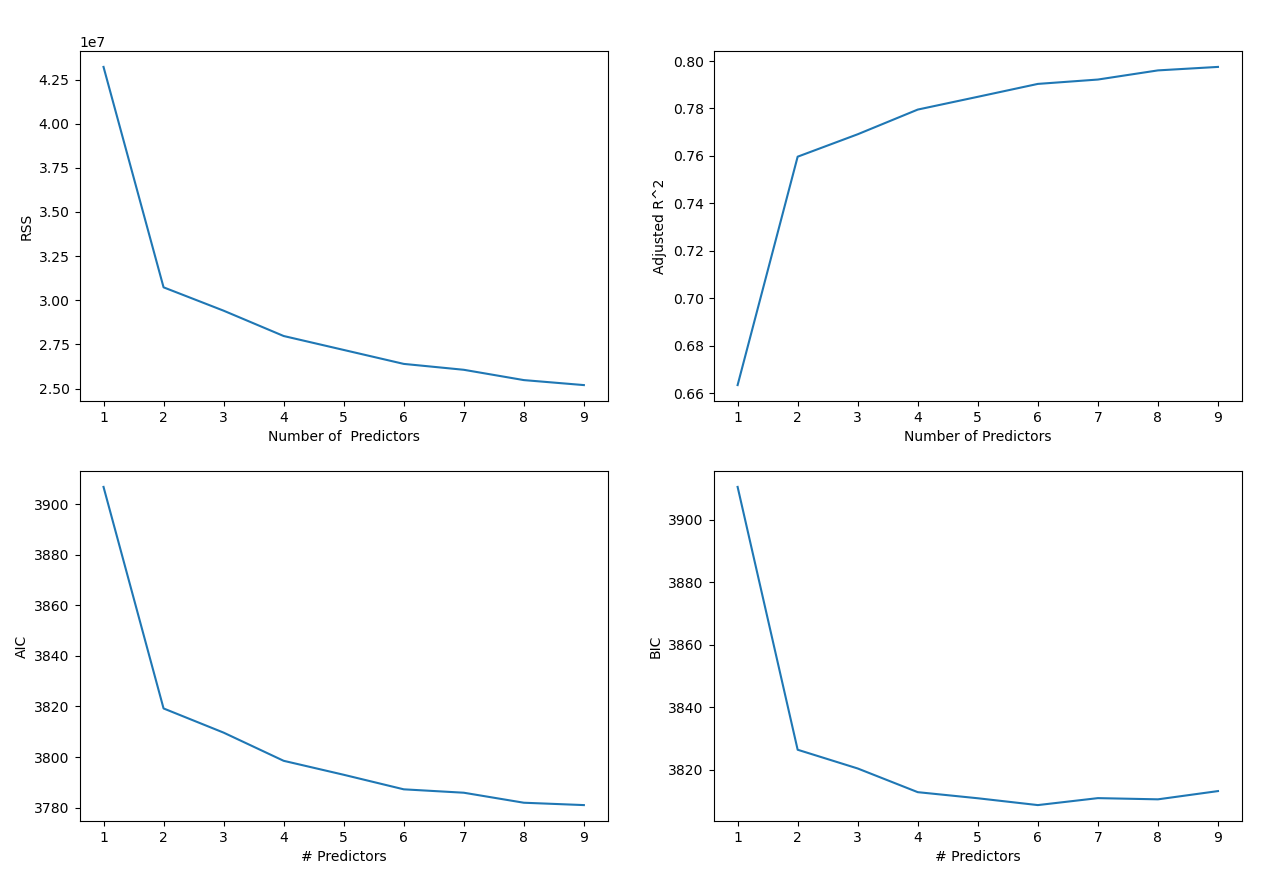
\includegraphics[width=12cm]{Img/Lab_6_5_1_plot.PNG}
	\caption{Lab 6.5.1 plotted results}
	\label{fig:Lab_6_5_1_plot}
\end{figure} 
